\documentclass[runningheads]{llncs}
%
\usepackage{graphicx}
% Used for displaying a sample figure. If possible, figure files should
% be included in EPS format.
\graphicspath{ {../plots/} }

\usepackage{calc}

% state diagrams
\usepackage{tikz}
\usetikzlibrary{automata, positioning, arrows}
\tikzset{
  initial text={},
  ->, % makes the edges directed
  node distance=3.0cm, % specifies the minimum distance between two nodes. Change if necessary.
  every state/.style={rectangle, thick, text width=5em, align=center}  % sets the properties for each ’state’ node
}

% tables
\usepackage{multirow}

\usepackage{hyperref}
% If you use the hyperref package, please uncomment the following line
% to display URLs in blue roman font according to Springer's eBook style:
\renewcommand\UrlFont{\color{blue}\rmfamily}

% references
\usepackage[numbers,sort]{natbib}
\bibliographystyle{splncs04}
% quotation
\usepackage{dirtytalk}

\begin{document}

%
\title{
Spatial Prisoner’s Dilemma: \\
Keep your enemies closer and be loud about it}
%
%\titlerunning{Abbreviated paper title}
% If the paper title is too long for the running head, you can set
% an abbreviated paper title here
%
\author{
Martin Toman\inst{1} \and
Neil Yorke-Smith\inst{1}\orcidID{0000-0002-1814-3515}
}
%
\authorrunning{M. Toman, N. Yorke-Smith}
% First names are abbreviated in the running head.
% If there are more than two authors, 'et al.' is used.
%
\institute{Delft University of Technology, The Netherlands}
%
\maketitle              % typeset the header of the contribution
%
%
%
\begin{abstract}
Under what conditions can cooperation emerge and how can we sustain it?
We build a computer simulation of a multi-agent spatial environment using Prisoner's Dilemma as the principal agent interaction.
We expand the model by allowing agents to remember defectors, abstain from interacting with them, and warn nearby agents---local reputation of each agent is created.
We find that local reputation works excellent in sustaining cooperation and punishing defection.
The size of agent memory and amount of gossip are not important factors,
only the range of gossip has to be greater than the agent movement speed.

\keywords{First keyword  \and Second keyword \and Another keyword.}
\end{abstract}
%
%
%
\section{Introduction}

How can we encourage and sustain cooperation?
We can model behaviour of selfish individuals with \say{Prisoner’s Dilemma}
and use it for \say{discovery of the precise conditions that are necessary and sufficient for cooperation to emerge}~\cite{Axelrod84}.
An agents has to expect that even a single defection can be infinitely punished by never again being cooperated with \cite{GRIM}.
Such a risk may just not be worth it.

In the next section we provide a short overview of related work and outline gaps in knowledge that we aim to fill; then follows methodology, results, discussion and conclusion.
%
%
%
\section{Related Work}
Prisoner's Dilemma is used to model agent behaviour when we care about promoting cooperation and all agents are acting selfishly.
Defectors can only be punished (or avoided) if they can be identified;
the main benefit of a reputation system---providing identity and behaviour history for agents.
This is why services like Ebay or Airbnb have a rating system in place.

Various reputation systems were shown to strongly boost cooperation \cite{simple-reputation, dong-reputation}~among~others.
\cite{strangers-gossip} investigated the effects of gossip between PD game participants on the cooperation levels and found a slight boost between gossiping agents.
\cite{public-private-monitoring} allowed game participants to report some information about their opponents to their future opponents, they suggest that \say{[the efficacy of communication in promoting cooperation] depends on the quality of platforms that store reported information.}
Similarly, \cite{cooperation-communication} allowed unrestricted non-binding communication between agents---the boost to the cooperation levels was more than when the volume of information was limited.

All of the studies mentioned above were carried out using human subjects as game participants; the group sizes were also kept relatively small with few rounds.
This made the results difficult to analyze and almost impossible to draw strong conclusions from.

We aim to conclusively find out if, and how well, local reputation---built up via gossip---promotes and sustains cooperation in Spatial Prisoner’s Dilemma and under what parameters does it yield optimal results.
%
%
%
\section{Methodology}
To evaluate the effectiveness of local reputation in enforcing cooperation we use a computer simulation of Spatial Prisoner’s Dilemma.
We base the simulation on the design of \cite{smaldino}.
Our hypothesis is that local reputation will drive the simulation towards a cooperator--only population and will be able to sustain it indefinitely.

The simulation is implemented in Python using the Mesa\footnote{\url{https://github.com/projectmesa/mesa}} framework and the complete source is available online (\url{https://github.com/tinybeachthor/IPD}).

\begin{figure}[h]
  \centering
  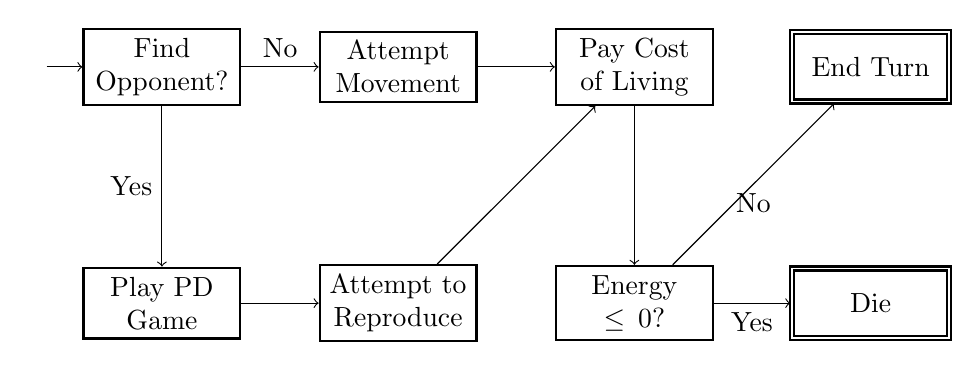
\begin{tikzpicture}

    \node[state, initial] (find_opponent) {Find Opponent?};

    \node[state, below of=find_opponent] (play) {Play PD Game};
    \node[state, right of=play] (reproduce) {Attempt to Reproduce};
    \node[state, right of=find_opponent] (move) {Attempt Movement};
    \node[state, right of=move] (cost) {Pay Cost of Living};
    \node[state, below of=cost] (energy) {Energy $\le 0$?};

    \node[state, accepting, right of=energy] (die) {Die};
    \node[state, accepting, above of=die] (end) {End Turn};

    \draw
      (find_opponent) edge[left] node{Yes} (play)
      (find_opponent) edge[above] node{No}  (move)
      (play) edge[] node{} (reproduce)
      (reproduce) edge[] node{} (cost)
      (move) edge[] node{} (cost)
      (cost) edge[] node{} (energy)
      (energy) edge[below] node{No}  (end)
      (energy) edge[below] node{Yes} (die)
      ;
  \end{tikzpicture}
  \caption{Agent behaviour diagram: showing the decision flow of an agent's single turn}
  \label{fig:agent_behaviour}
\end{figure}

Agent's behaviour is defined by the finite state diagram shown in Figure~\ref{fig:agent_behaviour}.
Every agent can play at most a single PD game in each time step.
Similarly, when no opponent is found, movement only happens if an empty cell is found nearby; if there is more than one empty cell, one is chosen at random.
A single round of the game is defined using a payoff matrix as shown in Table~\ref{table:payoff}, with $T > R > P > S$ and $2R > T + S$ \cite{chammah1965}.
Like in the original model \cite{smaldino},
we use $R = 3$, $T = 5$, $P = 0$.
We will determine value for $S$ empirically, in such a way it lead to total extinction quickly. This choice for the parameter will ensure that, if we reach cooperation, it was caused by the reputation mechanism;
and not because of random interactions in the model.

\begin{table}[h!]
  \caption{Payoff matrix}
  \label{table:payoff}

  \centering
  \begin{tabular}{c c||c|c}
    & & \multicolumn{2}{c}{Opponent's move} \\
    & & Cooperate & Defect \\
    \hline\hline

    \multirow{4}{6em}{Player's move}
    & \multirow{2}{5em}{Cooperate}
      & Player:\ \ \ \ \ \ R & Player:\ \ \ \ \ \ S \\
    & & Opponent: R & Opponent: T \\
    \cline{2-4}
    & \multirow{2}{5em}{Defect}
      & Player:\ \ \ \ \ \ T & Player:\ \ \ \ \ \ P \\
    & & Opponent: S & Opponent: P \\
  \end{tabular}
\end{table}

We expand the model by giving agents a (limited size) memory to keep track of past defectors and to allow them to actively and freely share this knowledge by gossiping with other agents in a given range.
The range at which agents can be contacted and the amount of information which agents provide will be varied.

To determine the effectives of gossip in promoting cooperation, we observe the rate of convergence to a population of cooperators, stopping the simulation once stable equilibrium is achieved.
The main properties measured about the model is the saturation of cooperator and defector populations.

Since we are simulating stochastic behaviour and we are interested in the converged outcomes,
we run every simulations 30 times for each parameter combination and we plot the standard deviations of the results.
We drop the 2 most extreme outliers, both positive and negative, from the plots; this allows us to show the behaviour of the model, devoid of unusual probabilistic anomalies.
To ensure integrity of the results, we check the outliers removed and investigate any unusual interactions for relevance to the results.

We also record characteristic patterns formed by the populations as influenced by different parameters.
We do this, because it was shown by earlier work \cite{spatial-patterns} that in Spatial Prisoner's Dilemma interesting patterns can emerge over time.
These patterns are very similar to patterns occurring in nature, which are often created by reaction--diffusion processes.
This suggests a deeper link between our model and biological activity.
%
%
%
\section{Results}
What follows is an impartial presentation of our simulation results.
A more thorough explanation of the data in the context of related research
is offered in the next section.

\subsection{Baseline model}
First we look at the plain model with 0-memory and no communication (gossip) between agents.
This is a replication of \cite{smaldino} on a smaller scale.

\begin{figure}[!ht]
  \centering
  \makebox[\textwidth]{
    \includegraphics[width=\textwidth]{saturation&S-memory0+gossip0_250steps_large}
  }
  \makebox[\textwidth]{
    \includegraphics[width=\textwidth]{saturation&S-memory0+gossip0_500steps_large}
  }
  \caption{Agent type saturation for various $S$ (sucker's payoff) after 250, 500 steps; SD of 30 simulation runs, outliers removed}
  \label{fig:agent_sat/S-memory0gossip0}
\end{figure}

We begin by exploring the robustness of the model against social harshness---represented by the $S$ (sucker's payoff) parameter.
In Figure~\ref{fig:agent_sat/S-memory0gossip0} we present the results of running the simulation for $2.5 \leq S \leq 0.0$.
We observe that $S = -1.5$ leads to total extinction in the model by step 500;
we use this value for further simulations to determine the effectiveness of memory and the gossip mechanism at promoting and sustaining cooperation.

\subsection{Gossip about defectors}
Next we enable communication between the agents.
We allow agents remember the 5 most recent defectors and to ask nearby agents in a Moore neighborhood of radius 1, 2, and 3 if they remember an agent defecting in a certain number of past encounters---varying between $0$ and $5$ (including both bounds).
We run the simulation for 1000 steps and plot the agent type saturations in Figure~\ref{fig:agent_sat/gossip_size_step1000}.

\begin{figure}[!h]
  \centering
  \makebox[\textwidth]{
    \includegraphics[width=\textwidth]{saturation&gossip_size-range1_1000steps_large.pdf}
  }
  \makebox[\textwidth]{
    \includegraphics[width=\textwidth]{saturation&gossip_size-range2_1000steps_large.pdf}
  }
  \makebox[\textwidth]{
    \includegraphics[width=\textwidth]{saturation&gossip_size-range3_1000steps_large.pdf}
  }
  \caption{Agent type saturation for various gossip sizes after 1000 steps, gossip radii 1, 2, and 3, respectively top to bottom; SD of 30 simulation runs, outliers removed}
  \label{fig:agent_sat/gossip_size_step1000}
\end{figure}

We found that the introduction of gossip is a strong deterrent of defection and leads to cooperator--only populations quickly.
The size of the memory and the size of the gossip are not significant factors, only speeding up the convergence slightly.
The most important factor in predicting cooperator success is the range of the gossip.

\subsection{Spatial patterns}

\begin{figure}[!hb]
  \centering
  \textbf{Baseline:} Memory size 0 - Gossip size 0 - Gossip range 0
  \makebox[\textwidth]{
    \includegraphics[width=\textwidth/4]{spatial-memory0+gossip0+range0.pdf}
    \includegraphics[width=\textwidth/4]{spatial-memory0+gossip0+range0-B.pdf}
    \includegraphics[width=\textwidth/4]{spatial-memory0+gossip0+range0-C.pdf}
  }
  \textbf{Final:} Memory size 1 - Gossip size 1 - Gossip range 3
  \makebox[\textwidth]{
    \includegraphics[width=\textwidth/4]{spatial-memory1+gossip1+range3-A.pdf}
    \includegraphics[width=\textwidth/4]{spatial-memory1+gossip1+range3-B.pdf}
    \includegraphics[width=\textwidth/4]{spatial-memory1+gossip1+range3-C.pdf}
  }
  \caption{Spatial patterns formed by agents after simulating for 500 steps, defectors are red, cooperators are green}
  \label{fig:spatial}
\end{figure}

We include images of the spatial patterns formed by the simulations in Figure~\ref{fig:spatial}.
Since the model has an inspiration in biology this is an interesting visualization to include.
We show 3 patterns formed after simulating for 500 steps for each of the following configurations
(these are the same as used in the sections above):
\begin{enumerate}
  \setlength\itemsep{0em}
  \setlength\parskip{0cm}
  \item
    \textbf{Baseline:} the base model, without any extensions (0-memory, no gossip)
  \item
    \textbf{Final:} every agent can remember the single last defector and gossip about it,
    radius of the gossip is 3 units in a Moore neighborhood
\end{enumerate}
%
%
%
\section{Discussion}
Looking back at the results we collected in the previous section;
now we present a more in-depth commentary on their meaning and
put them in a wider context.

We have seen that the baseline model act as expected and leads to total extinction quickly.
This is consistent with the behaviour observed by \cite{smaldino}.
Agents can prolong their existence if the cooperators are able to form a cluster,
but there is no escaping eventual extinction.

From \cite{simple-reputation, public-private-monitoring} we know that reputation systems promote cooperation.
We wanted to see if local reputation system suffices: we let agents communicate what they remember to nearby agents.
By allowing agents to let nearby agents know about the defectors they remember, we can consistently achieve cooperator--only population quickly.
The amount of the information included in the gossip is not very important, the main parameter is the range of the gossip.
By increasing it we can converge to cooperation faster.
%
%
%
\section{Conclusion}
We aimed to provide a definitive evaluating of the efficacy of local reputation---built up via gossip---in promoting and sustaining cooperation in selfish populations.
The inspiration came from many different papers taking various approaches to investigate effects of communication and reputation on cooperation in iterated exchange games.
The prior research has used human subjects in relatively small groups with few rounds of the game, the results achieved were difficult to analyze and to draw strong conclusions from.
To address this we use a computer simulation to evaluate effects of local reputation on the cooperation levels.

% final results
We found the most important factor in predicting cooperator success is the range at which gossip can be exchanged; the amount of information included in the gossip has negligible effect.
If the gossip can move faster than agents, cooperators will flourish. Otherwise, defectors can reach full population saturation.
From what we find, the best way to ensure cooperation (and survival of a population) is to keep your enemies close and be loud about it.
The louder the better.

% future work
Our simulation setup was limited in representing real world conditions.
We assumed all information is transferred with 100\% fidelity: no noise is present, no information is lost, all agents share all information openly.
As shown by \cite{noise}, not all strategies that perform well in noiseless environments can do so under the presence of noise.
Next, agents could be given probabilistic behaviour making the classification into cooperator/defector more complex: this would work against the gossip mechanism we used.
The gossip mechanism could turn out to be disadvantageous if the agent behaviour was random enough, since it would deter more cooperator--cooperator interactions.
%
%
%
% ---- Bibliography ----
%
\bibliography{references}

\end{document}
